% Arquitectura de sistema: nodo ESP32 <-> broker MQTT <-> backend FastAPI <-> dashboard React.
% Fuente de verdad: docs/hardware-spec.md (nombres de topics [CONFIRMAR] con firmware).
% Ancho natural <= 13.6 cm, sin escalar.
\documentclass[tikz,border=4pt]{standalone}
\usepackage[utf8]{inputenc}
\usepackage[T1]{fontenc}
\usepackage{lmodern}
\usetikzlibrary{shapes.geometric, arrows.meta, positioning, fit, backgrounds, calc}

\definecolor{acento}{RGB}{176,30,30}   % unico acento: lazo de actuacion (cmd)

\tikzset{
  base/.style     = {draw, thick, align=center, font=\fontsize{7.5}{8.5}\selectfont, inner sep=2pt,
                     minimum height=8mm},
  mcu/.style      = {base, very thick, fill=gray!28},
  process/.style  = {base, fill=gray!10, minimum width=22mm, text width=21mm},
  activo/.style   = {process, draw=acento, very thick},
  sombra/.style   = {process, dashed, fill=white},
  store/.style    = {base, cylinder, shape border rotate=90, aspect=0.18, fill=gray!18,
                     minimum width=22mm, text width=21mm, minimum height=10mm},
  ext/.style      = {base, dashed, fill=white},
  data/.style     = {-{Stealth[length=2mm]}, thin},
  cmdf/.style     = {-{Stealth[length=2.3mm]}, line width=1.1pt, acento},
  lbl/.style      = {font=\fontsize{7}{7.6}\selectfont, inner sep=1pt, align=left},
  capa/.style     = {font=\fontsize{7}{7.5}\selectfont\bfseries\scshape, text=gray!55!black,
                     rotate=90, inner sep=1pt},
  banda/.style    = {draw=gray!55, fill=gray!5, rounded corners=3pt},
}

\begin{document}
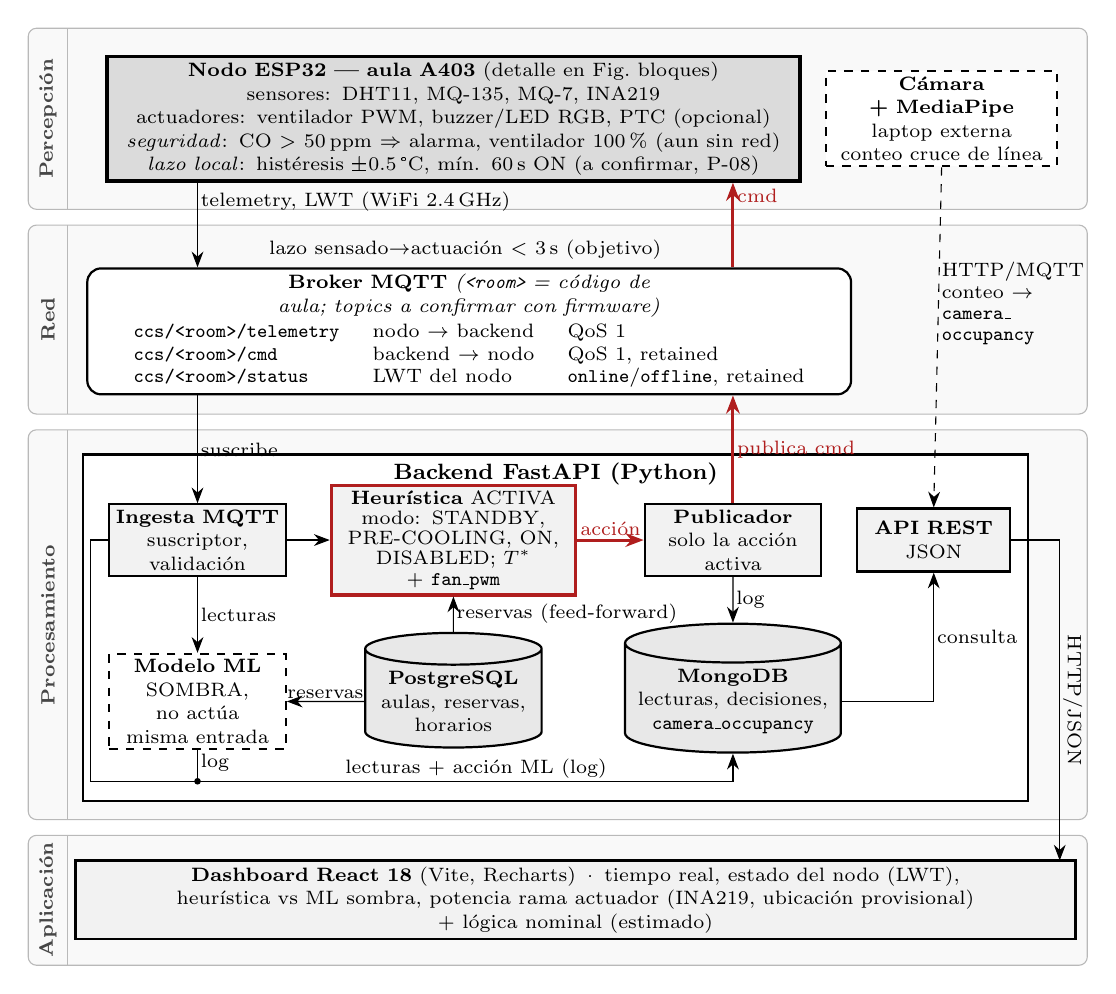
\begin{tikzpicture}

% ======== bandas de capas (rotulo vertical a la izquierda) ========
\begin{scope}[on background layer]
  \draw[banda] (-6.85, 1.30) rectangle (6.6,-1.00);
  \draw[banda] (-6.85,-1.20) rectangle (6.6,-3.60);
  \draw[banda] (-6.85,-3.80) rectangle (6.6,-8.75);
  \draw[banda] (-6.85,-8.95) rectangle (6.6,-10.60);
  \draw[gray!55] (-6.35,1.30) -- (-6.35,-1.00) (-6.35,-1.20) -- (-6.35,-3.60)
                 (-6.35,-3.80) -- (-6.35,-8.75) (-6.35,-8.95) -- (-6.35,-10.60);
\end{scope}
\node[capa] at (-6.60, 0.15) {Percepción};
\node[capa] at (-6.60,-2.40) {Red};
\node[capa] at (-6.60,-6.28) {Procesamiento};
\node[capa] at (-6.60,-9.77) {Aplicación};

% ======== Capa 1: nodo y camara ========
\node[mcu, minimum width=88mm, text width=86mm] (nodo) at (-1.45,0.15)
  {\textbf{Nodo ESP32 — aula A403} (detalle en Fig.~bloques)\\
   sensores: DHT11, MQ-135, MQ-7, INA219\\
   actuadores: ventilador PWM, buzzer/LED RGB, PTC (opcional)\\
   \textit{seguridad}: CO $>$ 50\,ppm $\Rightarrow$ alarma, ventilador 100\,\% (aun sin red)\\
   \textit{lazo local}: histéresis ±0.5\,°C, mín. 60\,s ON (a confirmar, P-08)};
\node[ext, minimum width=29mm, text width=28mm] (cam) at (4.75,0.15)
  {\textbf{Cámara}\\\textbf{+ MediaPipe}\\laptop externa\\conteo cruce de línea};

% ======== Capa 2: broker ========
\node[base, fill=white, rounded corners=5pt, minimum width=97mm, text width=95mm] (broker) at (-1.25,-2.55)
  {\textbf{Broker MQTT} \textit{(\texttt{<room>} = código de aula; topics a confirmar con firmware)}\\[1pt]
   \fontsize{7}{8}\selectfont
   \begin{tabular}{@{}l l l@{}}
   \texttt{ccs/<room>/telemetry} & nodo $\rightarrow$ backend & QoS 1\\
   \texttt{ccs/<room>/cmd}       & backend $\rightarrow$ nodo & QoS 1, retained\\
   \texttt{ccs/<room>/status}    & LWT del nodo               & \texttt{online}/\texttt{offline}, retained
   \end{tabular}};

% ======== Capa 3: backend ========
\node[base, fill=white, minimum width=120mm, minimum height=44mm, anchor=north] (be) at (-0.15,-4.10) {};
\node[font=\fontsize{8}{9}\selectfont\bfseries, anchor=north] at (be.north) {Backend FastAPI (Python)};

\node[process] (ing)  at (-4.70,-5.20) {\textbf{Ingesta MQTT}\\suscriptor, validación};
\node[activo, minimum width=31mm, text width=30mm, inner xsep=1pt, inner ysep=2pt, font=\fontsize{7}{7.3}\selectfont]  (heur) at (-1.45,-5.20) {\textbf{Heurística} ACTIVA\\modo: STANDBY,\\PRE-COOLING, ON,\\DISABLED; $T^{*}$\\+ \texttt{fan\_pwm}};
\node[process] (arb)  at ( 2.10,-5.20) {\textbf{Publicador}\\solo la acción\\activa};
\node[process, minimum width=19mm, text width=18mm] (api) at (4.65,-5.20) {\textbf{API REST}\\JSON};

\node[sombra, text width=21mm]  (ml)   at (-4.70,-7.25) {\textbf{Modelo ML}\\SOMBRA, no actúa\\misma entrada};
\node[store]   (pg)   at (-1.45,-7.25) {\textbf{PostgreSQL}\\aulas, reservas,\\horarios};
\node[store, minimum width=27mm, text width=26mm]   (mg)   at ( 2.10,-7.25) {\textbf{MongoDB}\\lecturas, decisiones,\\\texttt{camera\_occupancy}};

% nodo <-> broker <-> backend (verticales alineadas)
\draw[data] (ing.north |- nodo.south) -- node[lbl, right, pos=0.22] {telemetry, LWT (WiFi 2.4\,GHz)} (ing.north |- broker.north);
\draw[data] (ing.north |- broker.south) -- node[lbl, right] {suscribe} (ing.north);
\draw[cmdf] (arb.north |- broker.north) -- node[lbl, right, pos=0.85, text=acento] {cmd} (arb.north |- nodo.south);
\draw[cmdf] (arb.north) -- node[lbl, right, text=acento] {publica cmd} (arb.north |- broker.south);
\node[lbl, align=center] at ($(ing.north |- broker.north)!0.5!(arb.north |- broker.north)+(0,0.22)$)
  {lazo sensado$\rightarrow$actuación $<$ 3\,s (objetivo)};

% flujo interno
\draw[data] (ing) -- (heur);
\draw[data] (ing) -- node[lbl, right] {lecturas} (ml);
\draw[data] (pg) -- node[lbl, right, pos=0.5] {reservas (feed-forward)} (heur);
\draw[data] (pg) -- node[lbl, above] {reservas} (ml);
\draw[cmdf] (heur) -- node[lbl, above, text=acento] {acción} (arb);
\draw[data] (arb) -- node[lbl, right] {log} (mg);
% bus inferior hacia MongoDB: lecturas (Ingesta) + log del modelo en sombra
\coordinate (B) at ($(mg.south)+(0,-0.35)$);
\draw[data] (ing.west) -- ++(-0.22,0) |- node[lbl, pos=0.80, above] {lecturas + acción ML (log)} (B) -- (mg.south);
\draw (ml.south) -- node[lbl, right, pos=0.4] {log} (ml.south |- B);
\fill (ml.south |- B) circle (1.2pt);
\draw[data] (mg.east) -| node[lbl, pos=0.75, right] {consulta} (api.south);

% camara -> API (canal externo, valida ocupacion estimada por CO2)
\draw[data, dashed] (cam.south) -- node[lbl, right, pos=0.4] {HTTP/MQTT\\conteo $\rightarrow$\\\texttt{camera\_}\\\texttt{occupancy}} (api.north);

% ======== Capa 4: dashboard ========
\node[base, fill=gray!10, minimum width=127mm, text width=118mm, minimum height=10mm] (dash) at (0.10,-9.77)
  {\textbf{Dashboard React 18} (Vite, Recharts)\enspace·\enspace tiempo real, estado del nodo (LWT),
   heurística vs ML sombra, potencia rama actuador (INA219, ubicación provisional)\\+ lógica nominal (estimado)};
\draw[data] (api.east) -- (6.25,-5.20) -- node[lbl, rotate=-90, anchor=south, pos=0.5] {HTTP/JSON} (6.25,-9.27);

\end{tikzpicture}
\end{document}
